\documentclass{article}%
\usepackage[T1]{fontenc}%
\usepackage[utf8]{inputenc}%
\usepackage{lmodern}%
\usepackage{textcomp}%
\usepackage{lastpage}%
\usepackage{authblk}%
\usepackage{graphicx}%
%
\title{Differential regulation of Cu, Zn{-} and Mn{-}superoxide dismutases by retinoic acid in normal and psoriatic human fibroblasts}%
\author{Christina Cooley}%
\affil{Department of Laboratory Medicine, The First Affiliated Hospital of Sun Yat{-}sen University, Guangzhou, Guangdong, China}%
\date{01{-}01{-}2013}%
%
\begin{document}%
\normalsize%
\maketitle%
\section{Abstract}%
\label{sec:Abstract}%
A new study, in Cell Biology, reports that an enzyme called RIPE, which is essential for the production of dopamine D2{-}carboxylase and the dopamine receptor 2 etanergen, acts as a switch in an enzyme called STEPS (synthetic limonene lyase). Researchers put mice with different insulin sensitivity levels into two animals. In one they had two insulin levels on 50/50 and in the other they had 50/50 levels of STEPS. The control group showed even greater insulin sensitivity compared to this control group. Those with higher levels of STEPS actually had lower levels of the receptors that are produced in patients with type 1 diabetes.\newline%
As an added bonus, these mice had better insulin sensitivity for 20 months even after taking 7 antidepressants. Their insulin sensitivity improved at a rate that was 25 percent faster than the control group. Their insulin sensitivity increased until they reached 6.6 mmol/l and this is after two to 3 years. With the faster insulin response these mice still had less development of rheumatoid arthritis.\newline%
This whole surprise study adds to the growing body of research that suggest that even before a diabetic begins insulin therapy, the first step is insulin suppression. The importance of this in controlling diabetes is clear. It is now well established that the activity of STEPS is essential for insulin regulation. Whether it has an effect on insulin sensitivity, whether it has an effect on the development of diabetes, we just dont know yet. There is so much more that we still dont know, but it is becoming much more clear every day.

%
\subsection{Image Analysis}%
\label{subsec:ImageAnalysis}%


\begin{figure}[h!]%
\centering%
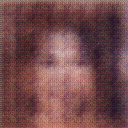
\includegraphics[width=150px]{500_fake_images/samples_5_193.png}%
\caption{A Black And White Cat Sitting In A Window Sill}%
\end{figure}

%
\end{document}